\section{Sicherheitsaspekte der Android-Architektur}

	Bereits durch die Architektur des Betriebssystems, insbesondere durch die restriktive Rechtevergabe und das Sandboxing, wird versucht, ein möglichst sicheres System bereitzustellen. Ab Android Version 4.3 kommt zusätzlich noch \textit{Security-Enhanced Linux (SELinux)} zum Einsatz.\\
	Verschlüsselungen und Signaturen werden Hardwareseitig durch eine \textit{Trusted Execution Environment (TEE)} unterstützt. TEE stellt einen besonders geschützten Bereich auf dem Prozessor dar, auf dem nur berechtige Anwendungen ausgeführt werden können, wie beispielsweiße die Verifikation des Bootmediums und Verschlüsselungsverfahren. Die Implementierung ist dabei Prozessor Hersteller abhängig - auf ARM wird dabei, wie bei iOS, auf \textit{TrustZone}\cite{TEE_ARM} zurückgegriffen.
	
	\subsection{Verifikation der Bootmedien} \label{sec:VerifikationDerBootmedien}
	Um bereits bei Systemstart eine Veränderung oder Ersetzung der Paritionen zu erkennen, wurde mit Android 4.4 eine Boot Verification eingeführt. Das Verfahren basiert auf der Funktion dm-verity des Device Mappers, welcher im Linux Kernel zu finden ist. Da diese Überprüfung durch den Kernel ausgeführt wird, muss vor dem Start von dm-verity erst der Bootloader und die Boot-Partition selbst auf ihre Integrität überprüft werden.
	Die Verifikation des Bootloaders ist nur schwer möglich, daher wird hierbei auf eine Hardware basierende root-of-trust, hier auf Basis des TEE, gesetzt. \\
	
	\subsubsection{Integritätscheck durch den Bootloader}
	Grundsätzlich ist Implementierung des Bootloader und dessen Vorgehen stark Geräteabhängig, daher werde ich hier im Folgenden lediglich das prinzipielle Vorgehen, welches durch das AOSP unterstützt wird, erläutern.\\
	Um die Boot- und Recovery-Partition (\textit{/boot, /recovery}) zu validieren gibt es zwei Möglichkeiten. Ist auf den beiden Partition jeweils ein offizielles Images des Smartphone Herstellers, kann auf einen OEM Key zurückgegriffen werden. Dieser ist in einem read-only in der Hardware festgeschrieben und wird vom Hersteller des Systems - zumeist der Smartphone Hersteller - festgelegt. Sollte eine Veränderung des Images vorgenommen worden sein, egal ob bewusst durch den Nutzer oder durch Schadcode, ist dieses Vorgehen nicht mehr möglich. Um aber dennoch eine Modifikation durch den Nutzer grundsätzlich zu ermöglichen, gibt es noch einen zweiten Weg. Dabei wird auf ein, in der Paritionssignatur gespeichertes, Zertifikat zurückgegriffen.\\\\
	Um zu unterscheiden ob ein offizielles oder inoffizielles Image erwartet wird, kann der Bootloader zwischen zwei Status unterscheiden:\\
	
	\begin{itemize}\itemsep0pt
		\item LOCKED - das aktuelle Boot-Image ist ein offizielles und kann mittels OEM Key verifiziert werden
		\item UNLOCKED - das aktuelle Boot-Image wurde verändert, und kann daher nicht mit dem OEM Key verifiziert werden
	\end{itemize}
	
\begin{flushleft}
	Diese und andere Versionsunabhängigen Informationen sind zwischen verschiedenen Images weites gehend gleich und werden daher auf einer extra Partition gespeichert (zumeist \textit{/misc}), welche somit im Falle eines Wechsel des Images nicht neu aufgesetzt werden muss.
\end{flushleft}
	 Wurde dies getan, wird beim Hochfahren immer eine Warnung ausgegeben, um den Nutzer darauf hinzuweisen, dass die Partition nicht mittels des festgeschrieben Keys verifiziert werden konnte. Daraus ergeben sich mehrere mögliche Zustände des Systems:\\\\
	
	\begin{figure}[h]
		\centering
		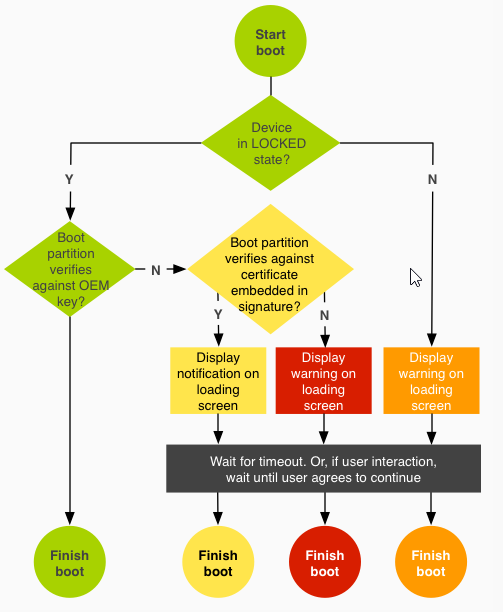
\includegraphics[width=0.7\linewidth, height=0.5\textheight]{android_pages/graphics/VerifiedBoot}
		\caption[Verified boot flow\protect\cite{VerifyingBoot}]{Verified boot flow\protect\cite{VerifyingBoot}}
		\label{fig:VerifiedBoot}
	\end{figure}
	
\begin{flushleft}
	Mit diesem Vorgehen wird auch die Integrität des Kernels sichergestellt, welcher in der \textit{/boot-} Partition abgelegt ist. Die Steuerung wird nach diesem Vorgang an den Kernel übergeben, welcher die Verifikation weiterer Partitionen übernimmt.\newline\\

	Um zu verhindern, dass Angreifer einfach den Bootloader manipulieren um an Daten heranzukommen, muss die Partition welche die Nutzerdaten beinhaltet (\textit{/userdata}) vor einer Veränderung an dem Bootsystem formatiert werden.
\end{flushleft}
	
	\subsubsection{Integritätscheck mittels dm-verity}
	Weitere Integritätschecks werden von der Kernelfunktion dm-verity übernommen.
	dm-verity arbeitet mit einem SHA-256 Hash-tree, der wie folgt aufgebaut ist:\\
	Für jeden 4K Sektor auf der Parition wird ein Hashwert berechnet. Jeweils zwei dieser Werte werden wiederum zu einem Neuen verrechnet. Dies wird solange wiederholt, bis nur noch ein Hashwert, der \textit{root-hash}, übrig ist. Um nun die Integrität sicherzustellen wird dieser root-hash, mit einem bereits berechneten Soll-Wert verglichen. Sind diese identisch, ist die Parition integer.
	
	\begin{figure}[h]
		\centering
		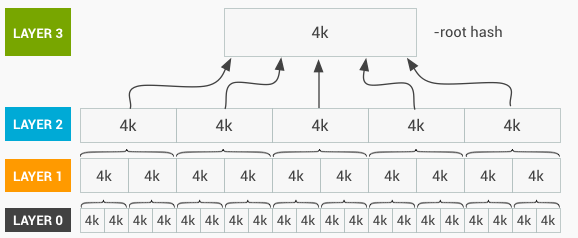
\includegraphics[width=0.7\linewidth]{android_pages/graphics/dm-verity-table}
		\caption[Aufbau des Hash-Trees]{Aufbau des von dm-verity erstellten Hash-Trees\protect\cite{VerifiedBoot}}
		\label{fig:dm-verity-table}
	\end{figure}
	
\begin{flushleft}
	Um Manipulationen am Soll-Wert zu unterbinden, wird der Hash-Tree und ein Salt mit einem RSA Schlüssel signiert. Der genutzte RSA Public Key wird in der Boot-Partition abgelegt. Der Hash-Tree und der Salt hingegen werden hinter dem letzten Datenblock auf die zu verifizierenden Partitionen geschrieben. Besonders geeignet ist dieses Verfahren für Read-Only Paritionen, wie die System-Partition (\textit{/system}) welche das Betriebssystem beherbergt.\\
	Welche Paritionen mittels vm-verity auf ihre Integrität überprüft werden sollen, wird über einen Eintrag zu der jeweiligen Partition in der fstab-Datei festgelegt.
\end{flushleft}

	\subsection{Basis Rechtesystem}\label{sec:BasisRechteSystem}
	Von Linux wurde auch das Basis-Rechtesystem Übernommen, allerdings wird es leicht abgewandelt genutzt. Anstatt das ein Nutzer - im Sinne von der Person, die das Gerät bedient - des Mobilsystems eine eindeutige User-ID (UID) zugewiesen bekommt, wird jede Applikation auf dem System als ein Nutzer angesehen und bekommt zur Installationszeit eine UID. Jeder Nutzer, und somit jede App, arbeitet grundsätzlich erst einmal nur innerhalb der ihm zugewiesenen virtuellen Maschine und dem damit verbundenen Dateisystem.\\\\
	Da es dennoch in vielen Fällen nötig ist, Daten zwischen verschiedenen Apps auszutauschen, gibt es mehrer Möglichkeiten dies zu tun. Die üblichen Wege wären Intends oder Contentprovider. Zusätzlich gibt es noch die Möglichkeit mehreren Apps dieselbe UID zuweisen zu lassen. Dies ist allerdings nur möglich, wenn die entsprechenden Applikationen mit dem selben Zertifikat signiert wurden und in deren Manifest Datei eine gemeinsame UID festgelegt wurde.
	Mittlerweile bieten die meisten Android Geräte auch einen Multiuser-Betrieb an. Da ein Linux-Nutzer eine (oder mehrere) Apps darstellt, wird um zwischen verschiedenen Endnutzern zu unterscheiden an die UID der Apps für jeden Endnutzer noch ein Prä- oder Suffix der den physikalischen Nutzer identifiziert hinzugefügt.\\
	Auch bekommt durch dieses Vorgehen jede Applikation ihren eigenen Speicherbereich, welcher nur für dieser zugänglich ist. Durch dieses Rechtesystem wird versucht sicherzustellen, dass kein Nutzerprogramm als \textit{root} ausgeführt wird.\\
	
	\subsection{SELinx in Android}
	Das \textit{Discretionary Access Control (DAC)} System des Linux Kernels lässt nur relativ grobe Einstellungen zu. Hat man beispielsweiße eine Applikation, die höhere Rechte für die Ausführung benötigt, so bekommt diese unter Nutzung von DAC oftmals noch zusätzliche Rechte, welche die App nicht haben sollte.\\
	Um dieses Problem zu beheben wird seit Android 4.4 zusätzlich zum DAC noch SELinux und dessen \textit{Mandatory Access Control (MAC)} System genutzt.\\	
	\begin{quote}
	SELinux operates on the ethos of default denial. Anything that is not explicitly allowed is denied.\cite{SELinuxAndroid}
	\end{quote}
\begin{flushleft}
	Dabei wird, sofern das DAC System einen Zugriff gewährt, das MAC System konsultiert und nur wenn dieses auch den Zugriff gewährt. Welche Rechte eine Applikation hat und welche nicht, wird unter SELinux in MAC Policies festgehalten.\\
	
	Dabei sind zwei Nutzungsmodi zu unterscheiden. Während im \textit{permissive mode} Regelverstöße nur geloggt werden, wird im \textit{enforcing mode} die strikte Einhaltung erzwungen. In den Versionen 4.3 bis exklusive 5.0 war der \textit{enforcing mode} nicht überall in Nutzung. Dies änderte sich mit Version 5.0, seit dem läuft nur noch dieser Modus.
\end{flushleft}
	
	\subsection{Sandboxing und Permissions} \label{sec:SandBoxingNPermissions}
	%Jede Applikation hat läuft in ihrer eigenen Sandbox. Die Sandbox umfasst den Schutz eines Speicherbereichs, des genutzten Arbeitsspeichers und aller Prozesse der in der Sandbox laufenden Anwendungen.
	Wie bereits erwähnt, laufen die Applikationen jeweils in ihrer eigenen Sandbox. Grundsätzlich ist die App damit erst einmal in ihrer Ausführung auf ihren Bereich beschränkt und kann nicht mit anderen Prozessen und Daten außerhalb interagieren. Dennoch ist es in den meisten Fällen sinnvoll mit Systemservices und Nutzerdaten zu interagieren, die nicht in der eigenen Sandbox verfügbar sind. Um solche Zugriffe zu regeln, werden sogenannte Permissions genutzt.
	
	\subsubsection{Sandboxing}
	Die Hauptmerkmale der Sandbox sind, dass Prozesse eines Nutzer nicht die eines anderen beeinflussen, noch auf dessen Arbeitspeicher oder App internen Dateien zugreifen können. Diese Beschränkungen werden durch in erster Linie durch das Berechtigungssystem des Kernels festgelegt und durch den Einsatz von SELinux unterstützt. Eine App hat einen persistenten Speicherbeich (\textit{Internal Storage}) in welchem nur diese Zugriffsrechte besitzt. Außerdem wird durch den Kernel eine Isolation der Prozesse geregelt. Die genutzte JVM wirkt nicht direkt am Sandboxing mit, dennoch wird durch diese eine weitere Abstraktionsebene eingeführt, welche die Möglichkeit bietet weitere Regelungen vorzunehmen. %\cite[S.26]{Drake2014} .
	
	\subsubsection{Permissions im Detail}
	Um nun die bestehenden Zugriffsrechte erweitern zu können, müssen die entsprechenden Rechte (Permissions) in der Manifest Datei deklariert und angefordert werden. Zu Installationszeit werden diese Permissions dem Nutzer angezeigt und dieser wird gefragt, ob er den Rechtswünschen der App zustimmt oder nicht. Dabei gilt das \textit{Alles-Oder-Nichts-Prinzip}, d.h. entweder bekommt die Anwendung alle Rechte oder keine - was eine nicht Installation zur Folge hat. Des weiteren können die Berechtigungen nach der Installation nicht mehr angepasst werden.	Berechtigungen sind beispielsweise für Zugriffe auf externe Speichermedien oder auch die Kamera nötig. Dabei ist allerdings zu beachten, dass die Permissions zum Teil sehr grob definiert sind. Wodurch für den Nutzer nicht unbedingt erkenntlich ist, welche Informationen eine App warum abgreift und ob die App wirklich Gebrauch des Rechts macht.\\\\
	Anhand der folgenden Permission lässt sich die daraus resultierende Problematik gut erkennen:\\
	RECORD\_AUDIO Permission:
	\begin{quote}
	Allows an application to record audio \footnote{https://developer.android.com/reference/android/Manifest.permission.html\#RECORD\_AUDIO}
	\end{quote} 
	Dabei ist für den Nutzer nicht sichtbar, wann eine Aufnahme läuft, ausser die Applikation stellt dafür einen Hinweis bereit - wobei hier die Frage ist ob dieser auch wirklich verlässlich ist. Stellt die App einen Service bereit, kann ein solcher Mitschnitt auch im Hintergrund geschehen, und damit auch während eines Telefonats. Die einzige Chance RECORD\_AUDIO zur Laufzeit zu unterbinden ist, den Service bzw. die App über den Anwendungsmanager zu beenden.	Ausnahmen für diese Problematik sind Module wie GPS, WLAN und Bluetooth. Diese kann der Nutzer des Geräts abschalten und damit den Zugriff darauf verweigern.
	Dennoch ist das Problem auf viele Permissions übertragbar.\\\\
	Systemintern werden Permissions durch Nutzergruppen im Linux Berechtigungssystem dargestellt\cite[S. 28]{Drake2014}. Jeder Linux-Nutzer wird allen Gruppen entsprechend der Berechtigungen zugewiesen.
	Mit Android 4.3 (Kitkat) wurde eine versteckte Einstellungs-Activity namens \textit{App Ops} eingeführt. Darin konnte man einsehen welche App, wann welche Permission genutzt hat, und dieser einzelne Rechte zu entziehen und wieder zu erlauben. Diese Funktion konnte nur durch das Anlegen eines Activity Shortcuts und der direkten Verwendung in einer App genutzt werden. Leider wurde diese versteckte Einstellung aus den nächsten Versionen entfernt - bis Android M. \cite{HiddenActivity} \\
	Für Android M wurde mittlerweile angekündigt, dass eine derartige Einstellung nun fest mit eingebaut sein wird.\cite{AndroidMPermission} Allerdings wird es wohl kein Update für ältere Versionen geben, wodurch das Problem in diesen bestehen bleibt.
	
	\subsubsection{Besonderheit: Systemapps}
	Apps der System Hersteller können Rechte besitzen, die für normale Anwendungen nicht verfügbar sind, um Basis Apps und Services bereitzustellen. Hierfür werden alle Hersteller Applikationen mit sogenannten \textit{Publisher Keys} signiert und bekommen ggf. im Kernel festgeschriebene UIDs zugewiesen, welche erweiterte Rechte besitzen.
	
	\subsection{Verschlüsselung}
	\subsubsection{Verschlüsselung von Datenträgern}
	Mit Android 3.0 (Honeycomb) wurde die Möglichkeit eingeführt, die userdata-Partition vollständig zu verschlüsseln (Fulldisk Encryption - FDE). Basis der Verschlüsselung ist, wie bei der Verifikation der Partitionen (\ref{sec:VerifikationDerBootmedien}), eine Funktion des Device Mappers - dm-crypt.\\\\
	Zum Ent-/Verschlüsseln wird der Blockchiffrenmodus \textit{Cipher Block Chaining (CBC)} mit einem zufällig generierten 128-Bit AES Schlüssel (Disk Encryption Key, \textit{DEK}) verwendet. Die Verschlüsselung erfolgt Sektorweise. Da nicht immer seriell aus dem Speicher gelesen wird, kann nicht nur ein Initialisationsvektor (\textit{IV}) für die komplette Ent- und Verschlüsselung genutzt werden. Daher wird stattdessen für jeden Sektor anhand eines, vom Disk Encryption Key abgeleiteten, Salts \textit{S} und der Sektornummer \textit{SN} ein eigener IV berechnet.\\
	Somit gilt:
\begin{center}
	\begin{math}
	IV(SN) = AES_{S}(SN)\end{math}, mit \begin{math}S = SHA256(DEK)
	\end{math}
\end{center}
\chapter{test}
	Diese Art des Berechnung für einen IV nennt sich \textit{Encrypted Salt-Sector Initialization Vector} unter Nutzung der Hashfunktion \textit{SHA256} (\textit{ESSIV:SHA256}).\cite[S. 259]{Elenkov2014} Das Nutzen dieses Verfahren in dieser Art und Weise schützt die Daten allerdings nicht vor Manipulationen, da keinerlei Integritätscheck vorgenommen wird. Es wurde bereits demonstriert, dass es möglich ist, in ein verschlüsseltes Ubuntu 12.04 eine Backdoor einzuschleusen. Da das von Ubuntu genutzte Verschlüsselungsverfahren zu dem von Android identisch ist, lässt sich dieser Angriff übertragen. \footnote{http://www.jakoblell.com/blog/2013/12/22/practical-malleability-attack-against-cbc-encrypted-luks-partitions}\\
	Um den Disk Encryption Key zu sichern, wird dieser mit einem 128-Bit AES Key Encryption Key (KEK) verschlüsselt. Der KEK wird von einem, durch den Nutzer bestimmtes, Passwort abgeleitet. In der Vergangenheit, bis einschließlich zur Version 4.3, wurde für die Ableitung der Algorithmus \textit{PBKDF2} mit 2.000 Iterationen genutzt. Zusätzlich wurde noch ein 128-Bit Salt verwendet, welcher einem Zufallsgenerator entstammt. Da PBKDF2 nicht mehr aktuellen Sicherheitsstandards entspricht, wird seit Android 4.4 \textit{scrypt} als Ableitungsfunktion genutzt. Der DEK wird in verschlüsselter Form, zusammen mit dem Salt, in den Metadaten der verschlüsselten Partition abgelegt. Um eine Veränderung des DEK zu verhindern, bzw. die Integrität des DEK feststellen zu können, wird ab Version 5.0 dieser mit einem Key (Hardware-Bound Key, HBK) aus der TEE signiert. \\\\
	Damit ergibt sich folgendes Vorgehen:
	\begin{quote}
		\begin{enumerate}
		   \item Generate random 16-byte disk encryption key (DEK) and 16-byte salt.
		   \item Apply scrypt to the user password and the salt to produce 32-byte intermediate key 1 (IK1).
		   \item Pad IK1 with zero bytes to the size of the hardware-bound private key (HBK). Specifically, we pad as: 00 || IK1 || 00..00; one zero byte, 32 IK1 bytes, 223 zero bytes.
		   \item Sign padded IK1 with HBK to produce 256-byte IK2.
		   \item Apply scrypt to IK2 and salt (same salt as step 2) to produce 32-byte IK3.
		   \item Use the first 16 bytes of IK3 as KEK and the last 16 bytes as IV.
		   \item Encrypt DEK with AES\_CBC, with key KEK, and initialization vector IV. 
	   \end{enumerate}
	   \footnote{https://source.android.com/devices/tech/security/encryption/index.html}
	\end{quote}
	Als Nutzerpasswort kann eine Pin oder ein klassisches Passwort dienen. Seit Version 5.0 ist es auch möglich ein Eingabemuster als Passwort zu nutzen. \\
	Ein Vorteil, der durch das nutzen eines KEK und eines DEK zustande kommt, ist der, dass bei einer Änderung des Nutzerpasswortes nicht die komplette Partition neu verschlüsselt werden muss, sondern lediglich der DEK. Android 5.0 Geräte werden mit dem ersten Start automatisch, unter Nutzung eines Standard Passwortes, verschlüsselt. 
	
	\subsubsection{Keystore Service}
	Die FDE greift auf Partitions- und damit auf der Geräteebene. Hat es Schadcode erst einmal in ein laufendes System geschafft, wird dadurch der Schutz aber nicht mehr sichergestellt. Um dennoch einzelne Daten auf der Anwendungsebene sicher speichern zu können, kann mithilfe der durch das Entwicklungsfr amework bereitgestellte \textit{Cryptography Service Provider (CSP)} zurückgreifen. CSP stellen Algorithmen und Bibliotheken zum ent-/verschlüsseln, sowie zur Sicherstellung der Integrität von Daten bereit. Sollten die CSP aus dem Android Framework nicht reichen, kann man externe Nachladen. Dabei sollte man darauf achten, dass diese aus vertrauenswürdigen Quellen stammen, da die Sicherheit stark von der Richtigkeit der eingesetzten Algorithmen abhängig ist. Übrig bleibt dabei noch die Problematik, wie die Schlüssel für die Verschlüsselungen gespeichert werden sollen. Hierfür ist, seit Android 1.6, im Kernel ein Credential Service implementiert. Die im Service gespeicherten Daten werden wiederum durch ein vom Endnutzer bereitgestelltes Password verschlüsselt. Das Passwort kann in Form eines Musters, PINs oder eines üblichen Text Passworts vorliegen. Jeder Nutzer hat nur Zugriff auf die Daten im Keystore, die auch von ihm angelegt wurden.\\\\	
	Bis zur Android Version 4.0 wurden in diesem Keystore jedoch nur Netzwerkschlüssel abgelegt werden. Mit Version 4.3 wurde als zusätzlichen Schutz hardwareseitige Unterstützung mithilfe der TEE eingebaut.

	